\documentclass[../main.tex]{subfiles}
\begin{document}
\subsection{Experimento 1}
Reacción de disolución del $KNO_3$ en $H_2O$:
\[ KNO_{3(s)} \rightarrow K^+_{(ac)} + NO^-_{3(ac)} \]
Para obtener la solubilidad, tenemos que convertir las proporciones 
de masa/1 $mL$ a masa/100 $g$.
\begin{equation} \label{sol_eq_1}
    S^{T\degree}_{KNO_3} = \frac{masa (g)}{1\:mL\:H_2O} \times \frac{100}{100} \times \frac{1\:mL\:H_2O}{1\:g\:H_2O}
\end{equation}
Usando la ecuación \ref{sol_eq_1} por cada temperatura:
\[
    S^{91\degree}_{KNO_3} = \frac{2.01 (g)}{1\:mL\:H_2O} \times \frac{100}{100} \times \frac{1\:mL\:H_2O}{1\:g\:H_2O}
\]
\[
    S^{91\degree}_{KNO_3} = 201
\]\[
    S^{85\degree}_{KNO_3} = \frac{1.52 (g)}{1\:mL\:H_2O} \times \frac{100}{100} \times \frac{1\:mL\:H_2O}{1\:g\:H_2O}
\]
\[
    S^{85\degree}_{KNO_3} = 152
\]\[
    S^{76\degree}_{KNO_3} = \frac{1.20 (g)}{1\:mL\:H_2O} \times \frac{100}{100} \times \frac{1\:mL\:H_2O}{1\:g\:H_2O}
\]
\[
    S^{76\degree}_{KNO_3} = 120
\]\[
    S^{54\degree}_{KNO_3} = \frac{1.00 (g)}{1\:mL\:H_2O} \times \frac{100}{100} \times \frac{1\:mL\:H_2O}{1\:g\:H_2O}
\]
\[
    S^{54\degree}_{KNO_3} = 100
\]

Con estos datos, realizamos la curva experimental de la solubilidad del $KNO_3$:
\bigskip
\begin{center} 
    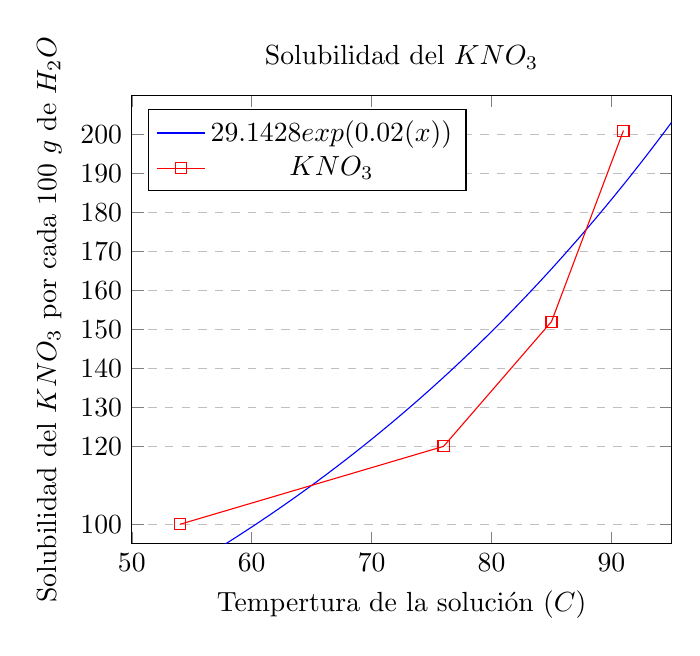
\begin{tikzpicture}
        \begin{axis}[
            title={Solubilidad del $KNO_3$},
            xlabel={Tempertura de la solución ($\degree C$)},
            ylabel={Solubilidad del $KNO_3$ por cada 100 $g$ de $H_2O$},
            xmin=50, xmax=95,
            ymin=95, ymax=210,
            xtick={50,60,70,80,90,100},
            ytick={100,120,130,140,150,160,170,180,190,200},
            legend pos=north west,
            ymajorgrids=true,
            grid style=dashed,
        ]
            %exponential function
            \addplot[
                domain=50:95,
                color=blue,
                samples=100
            ]{29.1428395077695*exp(0.020434940402*(x))};
            \addlegendentry{\(29.1428exp(0.02(x))\)}

            %data from table
            \addplot[
                color=red,
                mark=square,
            ]
            coordinates{ (54,100)(76,120)(85,152)(91,201)};
            \addlegendentry{$KNO_3$}
        \end{axis}
    \end{tikzpicture}
\end{center}

\subsection{Experimento 2}

Reacción del $H_2O$ con el $HCl$:
\[H_2O_{(l) \: + HCl_{(ac)} \rightarrow \: H_3O^+_{(ac)} \: + Cl^-_{(ac)}} \]

\subsection{Experimento 3}

\end{document}